

\documentclass[titlepage,usenames,a4,landscape,semhelv]{seminar}
\newcommand{\presenter}{Abram Hindle}
\newcommand{\conference}{Toronto Perl Mongers August 2010}
\newcommand{\gettitle}{Web Based Computer Music UIs with Mongrel2 and Harbinger}
\newcommand{\getmaintitle}{\gettitle}

\newcommand{\gettitleproper}{\gettitle}
\newcommand{\names}{Abram Hindle}
\author{
\names \\ 
{\small Toronto  Perl Mongers} \\
abram.hindle@softwareprocess.es
}



%%% Local Variables: 
%%% mode: latex
%%% TeX-master: t
%%% End: 

\usepackage{xspace,verbatim,listings}
%\slidewidth 300mm
\slideheight 200mm



\newcommand{\clstinline}[1]{\lstinline[language=c]!#1!}
\usepackage{graphicx}
\usepackage{comment}
%\usepackage[breaklines]{listings}
\usepackage{seminar}
\usepackage[usenames]{color} 
%\usepackage[pdftex]{color}
\usepackage{hyperref}
\input{seminar.bug}
\input{seminar.bg2}
\usepackage{tabularx}
\usepackage{fancyhdr}

\usepackage{graphicx}
\usepackage{amsmath}
\usepackage{amsfonts}
\usepackage{amssymb}
\usepackage{comment}
\usepackage{rotating} 
\usepackage{xspace}


\newcommand{\igh}[1]{
  \centering
  \includegraphics[height=0.9\textheight]{#1}
}
\newcommand{\igbigh}[1]{
  \centering
  \includegraphics[height=1.1\textheight]{#1}
}

\newcommand{\igwh}[1]{
  \includegraphics[width=0.4\textwidth]{#1}
}


\newcommand{\igw}[1]{
  \centering
  \includegraphics[width=0.9\textwidth]{#1}
}

\newcommand{\igws}[1]{
  \includegraphics[width=0.8\textwidth]{#1}
}

%WARNING THIS DOES A \newslide
% \renewcommand{\slideleftmargin}{-#1cm}        
\newcommand{\shiftleft}[2]{
        \newslide
        \renewcommand{\slideleftmargin}{-#1cm} 
        #2
        \newpage
        \leftmargin{0cm}
        \renewcommand{\slideleftmargin}{5mm}
}


\slidesmag{6}

\noxcomment
  \renewcommand{\slidetopmargin}{15.5mm}
  \renewcommand{\slidebottommargin}{13mm}

%  \renewcommand{\slidetopmargin}{20mm}

%  \renewcommand{\slidebottommargin}{20mm}
%  \renewcommand{\slidetopmargin}{15.5mm}
%  \renewcommand{\slidebottommargin}{13mm}

%  \renewcommand{\slideleftmargin}{0mm}
%  \renewcommand{\slideleftmargin}{-1cm}
\newcommand{\bitem}[1]{\item {\bf #1}: }
  %\renewcommand{\sliderightmargin}{1cm}
\newcommand{\catfile}[1]{ \newslide {\bf #1} 
	{\scriptsize 
		\tt 
		\lstinputlisting[language=PERL,breaklines=true]{#1} 
	} 
}
\newcommand{\sslide}[1]{ \newslide
	{\huge\bf #1}
}
\newcommand{\ttt}[1]{
	``{\tt #1}''
}





\title{\large \gettitleproper}
\renewcommand{\thetitle}{\gettitle}
\newcommand{\listperl}[1]{
	{\scriptsize
		\tt
	\lstinputlisting[language=PERL,breaklines=true]{#1}
	}
}
\newcommand{\listpython}[1]{
	{\scriptsize
		\tt
	\lstinputlisting[language=python,breaklines=true]{#1}
	}
}
\newcommand{\listjavascript}[1]{
	{\scriptsize
		\tt
	\lstinputlisting[language=HTML,breaklines=true]{#1}
	}
}

\newcommand{\listidl}[1]{
	{\scriptsize
		\tt
	\lstinputlisting[language=IDL,breaklines=true]{#1}
	}
}
\newcommand{\hrf}[1]{
	\href{#1}{#1}
}
%\newenvironment{notes}[0]{\tt \begin{note}}{ \end{note}  }

\newcommand{\softChange}{\textsf{softChange}\ }
\newcommand{\igColumnReal}[1]{\includegraphics[width=.9\textwidth]{#1}}
\newcommand{\igReal}[1]{\includegraphics[width=.9\textwidth]{#1}}
\markboth{ }{\presenter \thesection }

\newcommand{\albertaCVS}{\textsf{JReflex}\ }

% \fancyfoot[L]{\tiny \presenter}
% \fancyhead[L]{ \tiny \bf \gettitle}
% \fancyhead[R]{ \tiny \conference}
% \fancyfoot[R]{\tiny \thepage}

\newcommand{\fancyfootl}{\tiny \presenter}
\newcommand{\fancyheadl}{\tiny \bf \gettitle}
\newcommand{\fancyheadr}{\tiny \conference}
\newcommand{\fancyfootr}{\tiny \thepage}



\newcommand{\fancyempty}{
\renewcommand{\headrulewidth}{1.0mm}
\renewcommand{\footrulewidth}{0pt}
\fancyfoot[L]{}
\fancyfoot[R]{}
\fancyhead[L]{\fancyheadl}
\fancyhead[R]{\fancyheadr}
\renewcommand{\slidetopmargin}{15.5mm}
\renewcommand{\slidebottommargin}{13mm}
\renewcommand{\slidetopmargin}{0.5cm}
\renewcommand{\slidebottommargin}{3.0cm}
\renewcommand{\headsep}{0.0cm}
\renewcommand{\slideleftmargin}{5mm}
\renewcommand{\sliderightmargin}{0cm}

}
\newcommand{\fancyfancy}{
\renewcommand{\headrulewidth}{1.0mm}
\renewcommand{\footrulewidth}{1.0mm}
\fancyfoot[L]{\fancyfootl}
\fancyhead[L]{\fancyheadl}
\fancyhead[R]{\fancyheadr}
\fancyfoot[R]{\fancyfootr}
\renewcommand{\slidetopmargin}{15.5mm}
\renewcommand{\slidebottommargin}{13mm}


\renewcommand{\slidetopmargin}{0.5cm}
\renewcommand{\slidebottommargin}{0.5cm}



\renewcommand{\slideleftmargin}{5mm}
\renewcommand{\sliderightmargin}{0cm}

}

\fancypagestyle{empty}{\fancyempty}
\fancypagestyle{main}{\fancyfancy}

\fancyhf{}
\fancyfancy

\pagestyle{fancy}

\renewcommand{\headrulewidth}{1.0mm}
\renewcommand{\footrulewidth}{1.0mm}


\slideframe{none}
\renewcommand{\headwidth}{\textwidth}
\renewcommand{\slidetopmargin}{1.0cm}
\renewcommand{\slidebottommargin}{1.0cm}
%\renewcommand{\slidebottommargin}{2cm}
%\renewcommand{\slidebottommargin}{-0.1cm}


\newcommand{\igH}[1]{\includegraphics[height=.9\textheight]{#1}}
\newcommand{\igHh}[1]{\includegraphics[height=.5\textheight]{#1}}
\newcommand{\igHd}[1]{\includegraphics[height=.8\textheight]{#1}}
\newcommand{\igHq}[1]{\includegraphics[height=.25\textheight]{#1}}

\newcommand{\igW}[1]{}
\newcommand{\igWsixth}[1]{\includegraphics[width=.6\textwidth]{#1}}
\newcommand{\igWseventh}[1]{\includegraphics[width=.6\textwidth]{#1}}

\newcommand{\igWh}[1]{\includegraphics[width=.45\textwidth]{#1}}
\newcommand{\igWt}[1]{\includegraphics[width=.3\textwidth]{#1}}

\newcommand{\igWhalf}[1]{\includegraphics[width=.45\textwidth]{#1}}

\definecolor{source}{rgb}{1.0,0.7,0.0}
\definecolor{test}{rgb}{0.19,0.43,0.53}
\definecolor{build}{rgb}{0.73,0.0,0.50}
\definecolor{documentation}{rgb}{0.38,0.77,0.00}
\definecolor{doc}{rgb}{0.38,0.77,0.00}



\newcommand{\ess}[1]{\texttt{S#1}}
\newcommand{\dee}[1]{\texttt{D#1}}
\newcommand{\bee}[1]{\texttt{B#1}}
\newcommand{\tee}[1]{\texttt{T#1}}
\newcommand{\Apluss}{+}
\newcommand{\Aplus}{+}
\newcommand{\Aminus}{-}
\newcommand{\Aquest}{?}
\newcommand{\Aquestionbox}{?}
\newcommand{\Aequals}{=}
\newcommand{\Aequal}{=}

\newcommand{\hess}[1]{{\color{source}\texttt{S#1}}}
\newcommand{\hdee}[1]{{\color{doc}\texttt{D#1}}}
\newcommand{\hbee}[1]{{\color{build}\texttt{B#1}}}
\newcommand{\htee}[1]{{\bf\color{test}\texttt{T#1}}}

\providecommand{\macro}[2]{}
\renewcommand{\macro}[2]{
\providecommand{#1}{}
\renewcommand{#1}{#2}
}


\macro{\Apluss}{\textcolor[gray]{.80}{$\blacksquare$}}
\macro{\Aequal}{$\square$}
\macro{\Aminus}{\textcolor[gray]{.25}{$\blacksquare$}}

\macro{\Apluss}{{\color{red}{$\nearrow$}}}
\macro{\Aminus}{{\color{blue}{$\searrow$}}}
\macro{\Aequal}{{\color{green}{$\square$}}}
\macro{\Aplus}{\Apluss}

\macro{\Apluss}{{\color{red}{$\blacksquare$}}}
\macro{\Aminus}{{\color{blue}{$\blacksquare$}}}
\macro{\Aequal}{{\color{green}{$\square$}}}
\macro{\Aplus}{\Apluss}

\macro{\Apluss}{{\color{red}{$\blacksquare$}}}
\macro{\Aminus}{{\color{blue}{$\blacksquare$}}}
\macro{\Aequal}{{\color{green}{$\square$}}}
\macro{\Aplus}{\Apluss}
\definecolor{equal}{rgb}{0.9,0.0,0.9}
\macro{\Apluss}{{\color{red}{$\blacksquare$}}}
\macro{\Aequal}{{\color{equal}$\diamond$}}
\macro{\Aminus}{{\color{blue}{$\square$}}}
\macro{\Aplus}{\Apluss}
\macro{\Apluss}{{\color{red}{$\blacktriangleright$}}}
\macro{\Aequal}{{\color{equal}$\blacklozenge$}}
\macro{\Aminus}{{\color{blue}{$\blacktriangleleft$}}}

\providecommand{\questionbox}{}
\renewcommand*{\questionbox}{%
\ensuremath{\mathrel{\vcenter{%\offinterlineskip
\hbox{?}\vskip-1.5ex\hbox{$\square$}}}}}

\renewcommand*{\questionbox}{
\includegraphics[width=0.03\textwidth]{quest}
}

\macro{\Apluss}{{\color{red}{$\blacksquare$}}}
\macro{\Aminus}{{\color{blue}{$\square$}}}
\macro{\Aequal}{{\color{green}{$\boxtimes$}}}
\macro{\Aquest}{{\color{black}{$\questionbox$}}}

\macro{\Apluss}{{\color{red}{$\blacktriangle$}}}
\macro{\Aequal}{{\color{equal}$\square$}}
\macro{\Aminus}{{\color{blue}{$\blacktriangledown$}}}
\macro{\Aplus}{\Apluss}


\macro{\Aminus}{{\color{red}{$\blacktriangle$}}}
\macro{\Aequal}{{\color{equal}$\square$}}
\macro{\Apluss}{{\color{blue}{$\blacktriangledown$}}}
\macro{\Aplus}{\Apluss}
\macro{\Aequals}{\Aequal}

\macro{\Aplus}{\Apluss}


\macro{\Aplus}{\Apluss}




\macro{\esstxt}{\texttt{S}}
\macro{\teetxt}{\texttt{T}}
\macro{\deetxt}{\texttt{D}}
\macro{\beetxt}{\texttt{B}}

\providecommand{\ess}[1]{}
\providecommand{\tee}[1]{}
\providecommand{\dee}[1]{}
\providecommand{\bee}[1]{}
\renewcommand{\ess}[1]{\esstxt #1}
\renewcommand{\tee}[1]{\teetxt #1}
\renewcommand{\dee}[1]{\deetxt #1}
\renewcommand{\bee}[1]{\beetxt #1}

\providecommand{\pess}[1]{}
\providecommand{\ptee}[1]{}
\providecommand{\pdee}[1]{}
\providecommand{\pbee}[1]{}
\renewcommand{\pess}[1]{\ess{#1}}
\renewcommand{\ptee}[1]{\tee{#1}}
\renewcommand{\pdee}[1]{\dee{#1}}
\renewcommand{\pbee}[1]{\bee{#1}}

\macro{\essminus}{\ess{\Aplus}}
\macro{\teeminus}{\tee{\Aplus}}
\macro{\deeminus}{\dee{\Aplus}}
\macro{\beeminus}{\bee{\Aplus}}

\macro{\essplus}{\ess{\Aminus}}
\macro{\teeplus}{\tee{\Aminus}}
\macro{\deeplus}{\dee{\Aminus}}
\macro{\beeplus}{\bee{\Aminus}}

\macro{\essequal}{\ess{\Aequal}}
\macro{\teeequal}{\tee{\Aequal}}
\macro{\deeequal}{\dee{\Aequal}}
\macro{\beeequal}{\bee{\Aequal}}


\macro{\esspos}{\ess{\Aminus}}
\macro{\teepos}{\tee{\Aminus}}
\macro{\deepos}{\dee{\Aminus}}
\macro{\beepos}{\bee{\Aminus}}

\macro{\essneg}{\ess{\Aplus}}
\macro{\teeneg}{\tee{\Aplus}}
\macro{\deeneg}{\dee{\Aplus}}
\macro{\beeneg}{\bee{\Aplus}}

\macro{\deequest}{\dee{\Aquest}}

\macro{\x}{\xspace}

\newcommand{\ctest}{{\color{test} Test}\x}
\newcommand{\csource}{{\color{source} Source}\x}
\newcommand{\cdocumentation}{{\color{documentation} Documentation}\x}
\newcommand{\cbuild}{{\color{build} Build}\x}

\newcommand{\Major}{}
\newcommand{\Minor}{}
\renewcommand*{\Major}{\emph{Major}\x}
\renewcommand*{\Minor}{\emph{Minor}\x}

\newcommand{\transition}[2]{
}

\newcommand{\STD}{STD\xspace}
\newcommand{\ISTD}{ISTD\xspace}
\newcommand{\LSTD}{LSTD\xspace}
\newcommand{\VAR}{VAR\xspace}
\newcommand{\IVAR}{IVAR\xspace}
\newcommand{\LVAR}{LVAR\xspace}
\newcommand{\MED}{MED\xspace}
\newcommand{\IMED}{IMED\xspace}
\newcommand{\LMED}{LMED\xspace}
\newcommand{\AVG}{AVG\xspace}
\newcommand{\IAVG}{IAVG\xspace}
\newcommand{\LAVG}{LAVG\xspace}
\newcommand{\SUM}{SUM\xspace}
\newcommand{\ISUM}{ISUM\xspace}
\newcommand{\LSUM}{LSUM\xspace}
\newcommand{\LOC}{LOC\xspace}
\newcommand{\maintainability}{177741}
\newcommand{\cyclomatic}{mccabe}
\newcommand{\mccabe}{mccabe}
\newcommand{\halstead}{Halstead}
\newcommand{\mcc}{MCC\xspace}
\newcommand{\MCC}{MCC\xspace}
\newcommand{\HEFFORT}{HEFFORT\xspace}
 \newcommand{\HVOL}{HVOL\xspace}
\newcommand{\HDIFF}{HDIFF\xspace}
\newcommand{\HLEN}{HLEN\xspace}
\newcommand{\HVOCAB}{HVOCAB\xspace}

\newcommand{\igWsb}[1]{\noindent \includegraphics[width=1.0\textwidth]{#1}}
%\newcommand{\igWsb}[1]{\noindent \includegraphics[scale=1.5,origin=c]{#1}}
\usepackage{wrapfig}

\newenvironment{uquote}
{\list{}{\rightmargin -5em
         \leftmargin  -5em}
\item\relax}
{\endlist}

\newenvironment{specquoteaa}%
{\list{}{\rightmargin 0em%
         \leftmargin  5em}
\item\relax}
{\endlist}


\newenvironment{specquotea}%
{\list{}{\rightmargin 0em%
         \leftmargin  0em}
\item\relax}
{\endlist}

\newenvironment{specquoteb}%
{\list{}{\rightmargin 0em%
         \leftmargin  -1em}
\item\relax}
{\endlist}

\newenvironment{specquotec}%
{\list{}{\rightmargin 0em%
         \leftmargin  -2em}
\item\relax}
{\endlist}

\newenvironment{specquoted}%
{\list{}{\rightmargin 0em%
         \leftmargin  -3em}
\item\relax}
{\endlist}

\newenvironment{specquotee}%
{\list{}{\rightmargin 0em%
         \leftmargin  -4em}
\item\relax}
{\endlist}

\newenvironment{specquotef}%
{\list{}{\rightmargin 0em%
         \leftmargin  -5em}
\item\relax}
{\endlist}
\newenvironment{specquoteg}%
{\list{}{\rightmargin -1em%
         \leftmargin  -6em}
\item\relax}
{\endlist}

\newenvironment{specquotega}%
{\list{}{\rightmargin -1em%
         \leftmargin  -6.5em}
\item\relax}
{\endlist}


\newenvironment{specquoteh}%
{\list{}{\rightmargin -1em%
         \leftmargin  -7em}
\item\relax}
{\endlist}
\newenvironment{specquotei}%
{\list{}{\rightmargin -1em%
         \leftmargin  -8em}
\item\relax}
{\endlist}
\newenvironment{specquotej}%
{\list{}{\rightmargin -1em%
         \leftmargin  -9em}
\item\relax}
{\endlist}
\newenvironment{specquotek}%
{\list{}{\rightmargin -1em%
         \leftmargin  -10em}
\item\relax}
{\endlist}

%\newcommand{ninetyimage}[2]{%
%\begin{specquoted}
%\begin{center}
%\includegraphics[width=0.9\textwidth]{#1}\\
%#2
%\end{center}
%\end{specquoted}
%}





% \newenvironment{specquote}[1]%
% {\list{}{\rightmargin #1%
%          \leftmargin  0em%
% }
% \item\relax}
% {\endlist}



\newenvironment{uuquote}
{\list{}{\rightmargin 0em
         \leftmargin  0em}
\item\relax}
{\endlist}


\newcommand{\igbigslide}[1]{
\begin{uquote}
\newpage
%\centerslidesfalse
\fancyempty
\noindent
\begin{center}
\includegraphics[width=1.25\textwidth]{#1}
\end{center}
\newpage
\fancyfancy
%\centerslidestrue
\end{uquote}
}

\newcommand{\igbigslidecap}[2]{
\begin{uquote}
\newpage
%\centerslidesfalse
\fancyempty
\noindent
\begin{center}
\includegraphics[width=1.25\textwidth]{#1}
#2
\end{center}
\newpage
\fancyfancy
%\centerslidestrue
\end{uquote}
}


\newcommand{\igninetycap}[2]{
\begin{specquoted}
\begin{center}
\includegraphics[width=0.9\textwidth]{#1} \\
#2
\end{center}
\end{specquoted}
}
\newcommand{\igHninetycap}[2]{
\begin{specquoted}
\begin{center}
\includegraphics[height=0.9\textheight]{#1} \\
#2
\end{center}
\end{specquoted}
}
\newcommand{\igHeigthyfivecap}[2]{
\begin{specquoted}
\begin{center}
\includegraphics[height=0.85\textheight]{#1} \\
#2
\end{center}
\end{specquoted}
}



\newcommand{\igonecap}[2]{
\begin{specquoted}
\begin{center}
\includegraphics[width=\textwidth]{#1} \\
#2
\end{center}
\end{specquoted}
}
\newcommand{\igbigcap}[2]{
\begin{specquotee}
\begin{center}
\includegraphics[width=1.10\textwidth]{#1} \\
#2
\end{center}
\end{specquotee}
}
\newcommand{\igbigcapb}[2]{
\begin{specquotef}
\begin{center}
\includegraphics[width=1.25\textwidth]{#1} \\
#2
\end{center}
\end{specquotef}
}

\newcommand{\igbigcapc}[2]{
\begin{specquoteg}
\begin{center}
\includegraphics[width=1.25\textwidth]{#1} \\
#2
\end{center}
\end{specquoteg}
}


\newcommand{\igbigthirtycapb}[2]{
\begin{specquotei}
\begin{center}
\includegraphics[width=1.30\textwidth]{#1} \\
#2
\end{center}
\end{specquotei}
}

\newcommand{\igbigthirtyfivecapb}[2]{
\begin{specquotei}
\begin{center}
\includegraphics[width=1.35\textwidth]{#1} \\%
%#2
\end{center}%
\end{specquotei}
\begin{center}
#2
\end{center}
}


\newcommand{\bigslide}[1]{
\begin{uuquote}
\newpage
\centerslidesfalse
\fancyempty
#1
\newpage
\fancyfancy
\centerslidestrue
\end{uuquote}
}


\newcommand{\imageslide}[2]{
\newslide
\includegraphics[width=0.9\textwidth]{#2}
}

\newcommand{\figcaption}[1]{
\begin{center}
#1\\
\end{center}
}


\newcommand{\ig}[1]{\includegraphics{#1}}
%%%%%%%%%%%%%%%%%%%%%%%%%%%%%%%%%%%%%%%%%%%%%%%%%%%%%%%%%%%%%%%%%%%%%%%%%%%%%%%%
\begin{document}
\pagestyle{fancy} %bars..
\begin{slide}

\begin{center}
{\bf \LARGE \getmaintitle }

{\names } 

{\small Toronto Perl Mongers} \\
abram.hindle@softwareprocess.es



\end{center}


=Introduction
* What if we could use familar interfaces to make music
* Could we co-opt other software and events to produce musical events?
* Could we even use web interfaces and use javascript UIs?

=Imagine
* Extending your spread sheet into a soundboard or drum kit
* Turning your paint program into a violin
* Sonifying a boring website like ebay
* Taking a flash game, a SVG program, or HTML5 program and using it as
computer music input.

=Lets Hijack Something
* JS1k (js1k.org) demos (now)
* Javascript programs (now)
* Websites

=What am I talking about
* Abram will now show a demo of filler creep sonified

=What was that?
* Javascript game using Canvas
* Instrumented to send XMLHttpRequests to a mongrel2 server
* Mongrel handler communicates to Harbinger
** Who munges messages, massages them and hands them to:
* CSound receives messages from Harbinger.

=Ok.. but how do we communicate from Gnumeric?
* Harbinger!
** C Library for sending messages
*** Just embed calls from within another program
** A middle man
*** receives these messages
*** Delegates messages to other programs like CSound

\newslide

\begin{figure}
  \centering
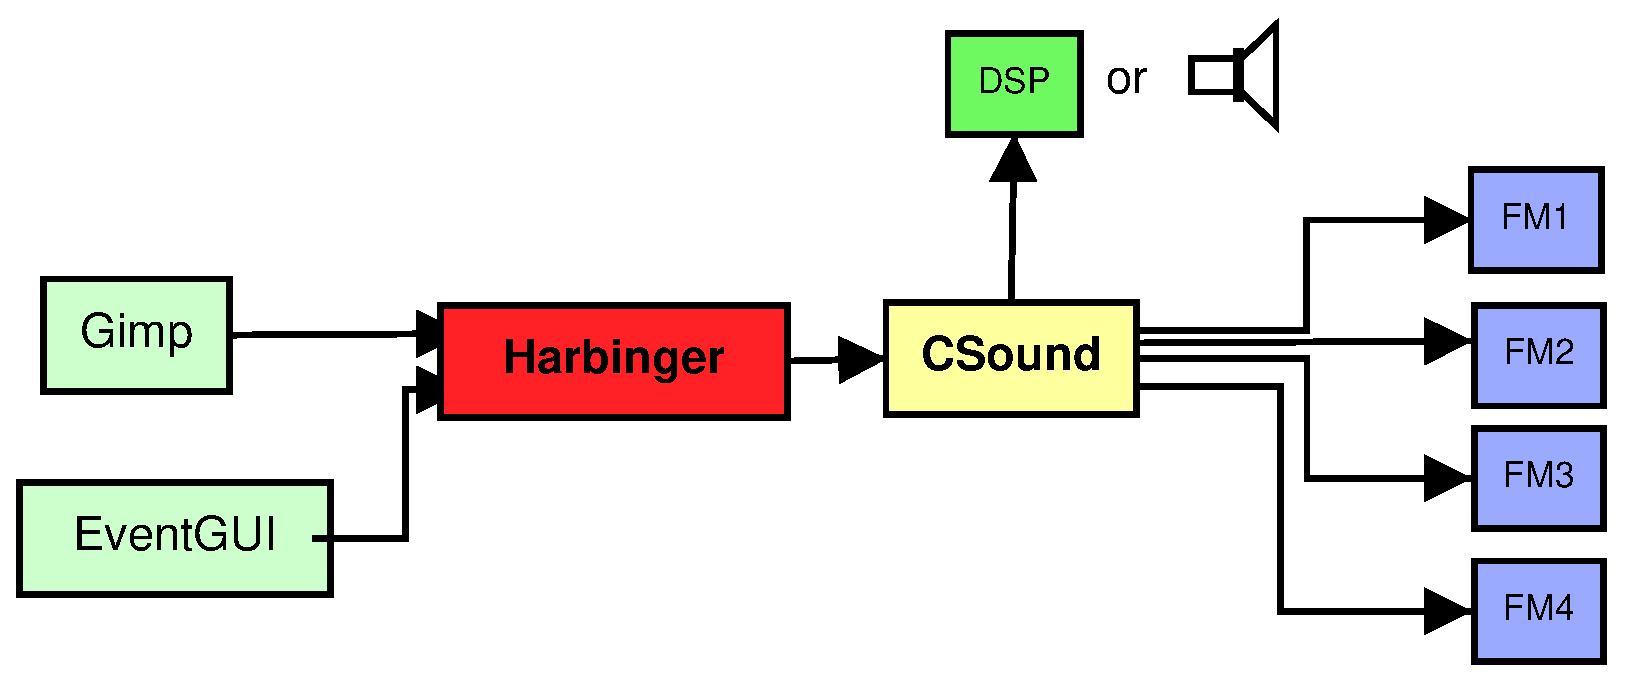
\includegraphics[width=\textwidth]{harbinger}  
\end{figure}


\newslide

\begin{figure}
  \centering
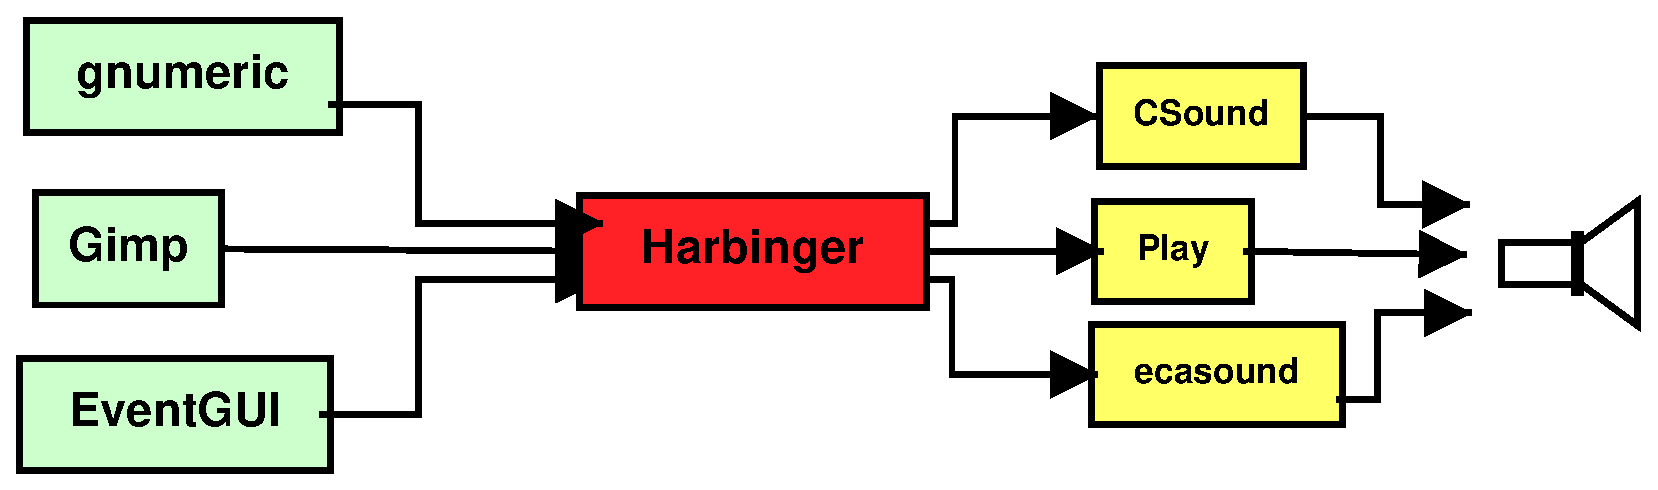
\includegraphics[width=\textwidth]{harbinger-example}
\end{figure}


=Harbinger
* send connectionless messages encoded in plain text
** UDP
* middle man routes these messages, and massages them
** Add code to the middle man to filter messages
* middle man passes messages on to other programs
 
=Why not OSC?
* OSC wasn't around or popular the time
* This is very simple
* This is very easy
* I can do more than OSC
* No errors if there is no one receiving the message
* Reduce dependencies.

=Gnumeric
* First configure and compile it
** \texttt{./configure --prefix=whereuwant it}
** \texttt{make \&\& make install}

=Gnumeric
* So we want to see when a cell is selected or when the current cell changes.
** grep for select, cell, update, change
* Cells are parts of sheets maybe look for that too

=Gnumeric
* Interesting procs
** scg\_object\_select
** scg\_cursor\_move
*** moves cursor down :(
*** but calls sv\_cursor\_set

=Gnumeric Guts
* look for sv\_cursor\_set
** src/sheet-view.c:sv\_cursor\_set
** sv\_cursor\_set does place the cursor 
*** sv\_set\_edit\_pos looks interesting though
** Lets change sv\_cursor\_set

=Gnumeric Debugging
* added code to src/sheet-view.c
** printed the view's current selection position
** Good
** This itself could be an instrument but I don't think it is enough

=Gnumeric: Get a Cell
* lets get a Cell Value
* Look in sheet-view.h, there must be a spreadsheet in there
** Yep sheet is in in sheet-view
** Lets look at sheet.h and see how to get a cell
*** \texttt{GnmCell  *sheet\_cell\_get(Sheet const *sheet, int col, int row);}
*** This looks good..

=Gnumeric: Cells
* Journey to gnumeric.h
** Where is \_GnmCell defined?
*** cell.h and cell.c
**** gnm\_cell\_get\_rendered\_text ?

=Gnumeric: Cells
* Added 
  \texttt{puts( gnm\_cell\_get\_rendered\_text( sheet\_cell\_get( sv->sheet,sv->edit\_pos.col, sv->edit\_pos.row)));}
** Got
\texttt{** (lt-gnumeric:5366): CRITICAL **: gnm\_cell\_get\_rendered\_text: assertion `cell != NULL' failed ERROR}
*** Although it did print values if it had them
*** Need to add a null check

=Gnumeric: Harbinger
* Now lets use the Harbinger API
* Remember to compile with -LHarbinger


=OpenArena
* Free datafiles
* IOQuake3 Engine

=Quake 3/IOQuake3/OpenArena
* Not the easiest to modify
** Contrary to existence of mods
* Useful events
** Gun fire
** Collisions
** Moving
** Rocket/Bullet Trails

=What to look for
* Sound system events
* Collision events
* Ricochets

=Quake 3 Arch notes
* Client and Server
* Game can be
** Native Game Code
** VM Code (QuakeC)
*** VM Code can't call POSIX :(

=Quake 3 Craziness
* To deal w/ the VM
** Anything that crosses the control/environment boundary
*** calls a syscall
* iD overloaded syscall with their own assembler based implementation
** wow 

=Quake 3
* Easiest for us to direct modify Quake3
* Compile to native code
* Ignore the VM

=Run IOQuake with our mods
*  \begin{verbatim}
     make && \
     cd ./build/release-linux-x86_64/ && \
     ./ioquake3.x86_64 +set sv_pure 0 \
     +set vm_cgame 0 +set vm_game 0 \ 
     +set vm_ui 0 +set s_initsound 0
\end{verbatim}


\begin{comment}
     Syscalls are good?
     openarena needs ioquake
     copy the baseq files to ioquake
     so openarena is for data files
     ioquake3 for code versio 1107 I think
     also applied some openarena patches
     to run quake I goto file:/home/abez/Desktop/quake3/ioquake3 and type
     make ; cd build/release-linux-x86_64/ ; ./*smp*64* +set s_initsound 0 ; cd .. ; cd ..
     our instrument:
     file:/home/abez/projects/Harbinger/quake3-2.pl
     cgame often gets compiled as a VM, we have to figure out how to compile cgame into a vm
     and then load it..
     essentially make a cgame mode
     then probably have a syscall which accesses it
     the server might have the same problem
     although shoving stuff in the server would make a lot of sense since it runs once.
     in client there is cg_syscall or something which catches syscalls then does a big case statement
     thus a true blue mod would probably help alot although it might limit the ability to play..
     a good idea would be to talk to ioquake people
     make && ./build/release-linux-x86_64/ioquake3.x86_64 +set sv_pure 0 +set vm_cgame 0 +set vm_game 0 +set vm_ui 0 +set s_initsound 0
     changed build to not make the vm..
     file:/home/abez/projects/Harbinger
     file:/projects/harbinger-quake3/quake3/ioquake3

\end{comment}

=Other suggestions
* GIMP, paint programs have nice UIs with lots of inform and tools.
* Instant Messaging
* follow strace
* follow tcpdump
* preload lib hooks and wrap calls


=Future Work
* Fish or Cut Bait?
** Work on music
** Work on tools?
** Restrictions versus freedom
* Other UIs

=Conclusions
* Take home:
** leverage the UIs of other software to produce music
*** avoid wasting your time reinventing the wheel
** Perl is the great glue that holds systems together
** avoiding complication helps for development speed
*** Hurts for performance (sometimes)


=
\end{slide}


\end{document}
